\documentclass[12pt]{article}
\usepackage[utf8]{inputenc}
\usepackage{caption}
\usepackage{times}
\usepackage{graphics}
\usepackage{graphicx}
\usepackage{float}
\usepackage{hyperref}
\usepackage{listings}
\lstset{
	basicstyle=\ttfamily,
	columns=fullflexible,
	frame=single,
	breaklines=true,
	postbreak=\mbox{\textcolor{red}{$\hookrightarrow$}\space},
}
\hypersetup{
	colorlinks=true,
	linkcolor=blue,
	filecolor=magenta,      
	urlcolor=cyan,
}

\title{Docker inrichten}
\author{Thomas van Dongen, Koen Schilders}
\date{28 februari 2018}

\begin{document}


% De titelpagina
\begin{titlepage}
\maketitle
\end{titlepage}



% Hier wordt beschreven hoe we Docker opzetten voor CI/CD
% Link naar tutorial: https://blog.philipphauer.de/tutorial-continuous-delivery-with-docker-jenkins/
\section{Opzet CI/CD met Docker}
Voor deze opdracht moeten we een CI/CD pipeline opzetten met Docker. De pipeline bestaat uit twee Docker containers. De ene container test de build en maakt een Docker image, de andere container deployed de container en draait de applicatie. Voor het testen maken we gebruik van Jenkins, en GlassFish wordt gebruikt om de applicatie te draaien. GlassFish heeft toegang tot de build files omdat deze door de Jenkins-container worden opgeslagen op de host-VM. De pipeline is uitgewerkt in \figurename \ref{fig:cicd_pipeline}.
\newline
\begin{figure}[H]
	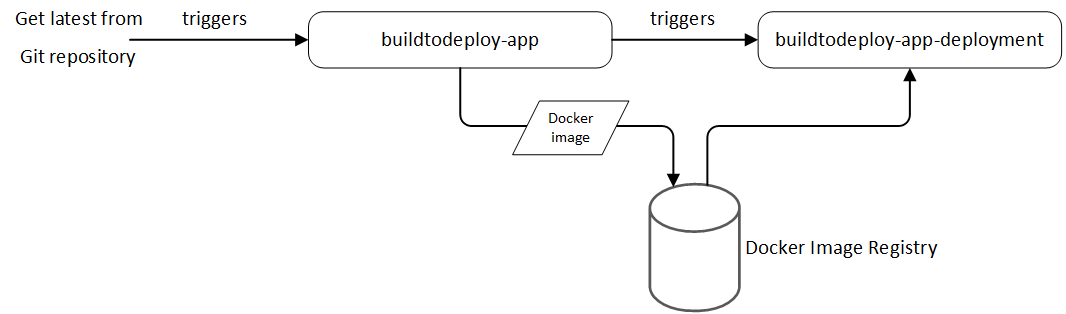
\includegraphics[width=\textwidth]{images/DockerPipeline.png}
	\caption{De pipeline van Docker containers\label{fig:cicd_pipeline}}
\end{figure}

\subsection{Git repository}
Eerst gaan we een Git repository maken met een kleine web-applicatie. De applicatie is een webpagina met enkele JUnit-tests voor back-end logica. Deze logica wordt niet gebruikt in de webpagina, en is alleen bedoeld om JUnit-tests aan te tonen (Figure \ref{fig:calculator_app}).

\begin{figure}[H]
	\begin{center}
		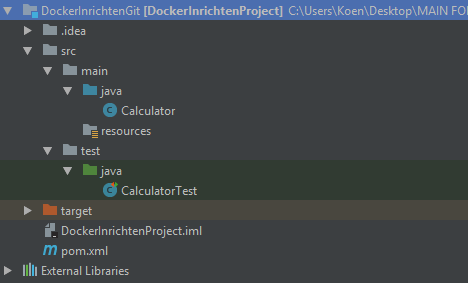
\includegraphics[width=0.5\textwidth]{images/CalculatorApplication.png}
		\caption{De structuur van de Calculator applicatie\label{fig:calculator_app}}
	\end{center}
\end{figure}

De Git repository heeft alleen een master branch. Dit is prima voor nu, maar in een echt project is het beter om het systeem van branches uit het releaseplan te gebruiken. Dat branchsysteem is ingericht voor CI/CD gebruik.

\subsection{Jenkins container}
Nu gaan we een Docker container maken waar Jenkins op draait. Deze moet zo worden ingericht dat Jenkins de Git repository weet te vinden, de tests gedraaid worden, en uiteindelijk een nieuwe Docker container aanroept.
\linebreak
In plaats van op een schone container Jenkins te installeren maken we gebruik van de kracht van Docker. Op de Docker Hub is een kant-en-klare Jenkins image te vinden. Deze kan gepulled worden met het volgende commando:

\begin{lstlisting}[language=Bash]
docker pull jenkins/jenkins
\end{lstlisting}

\noindent We kunnen de image openen met het volgende commando\textsuperscript{\cite{jenkins_documentation}}:

\begin{lstlisting}[language=Bash]
docker run -p 8080:8080 -p 50000:50000 -v jenkins_home:/var/jenkins_home jenkins/jenkins:latest
\end{lstlisting}

\noindent De docker instance draait, en heeft poort 8080 gemapped, zoals we hadden meegegeven in het commando. Nu moeten we Jenkins configureren. Hiervoor moet een wachtwoord ingevoerd worden, welke te vinden is in de console window.

Nu kunnen we Jenkins configureren. Eerst moeten we aangeven waar de git repository staat:

\begin{figure}[H]
	\begin{center}
		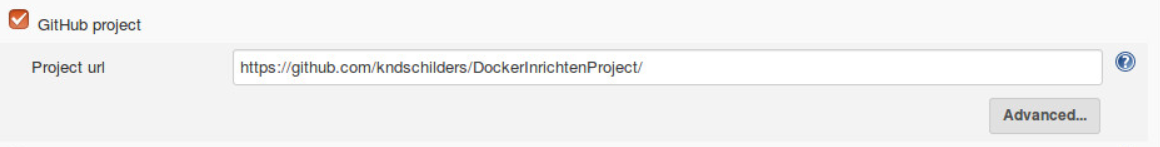
\includegraphics[width=1.0\textwidth]{images/Jenkins-Github.PNG}
		\caption{GitHub repository instellen\label{fig:jenkins_config_repo}}
	\end{center}
\end{figure}

\noindent Jenkins heeft user credentials nodig, en moet weten van welke branch hij de applicatie moeten halen. Deze credentials kunnen iets lager op de pagina ingevuld worden:

\begin{figure}[H]
	\begin{center}
		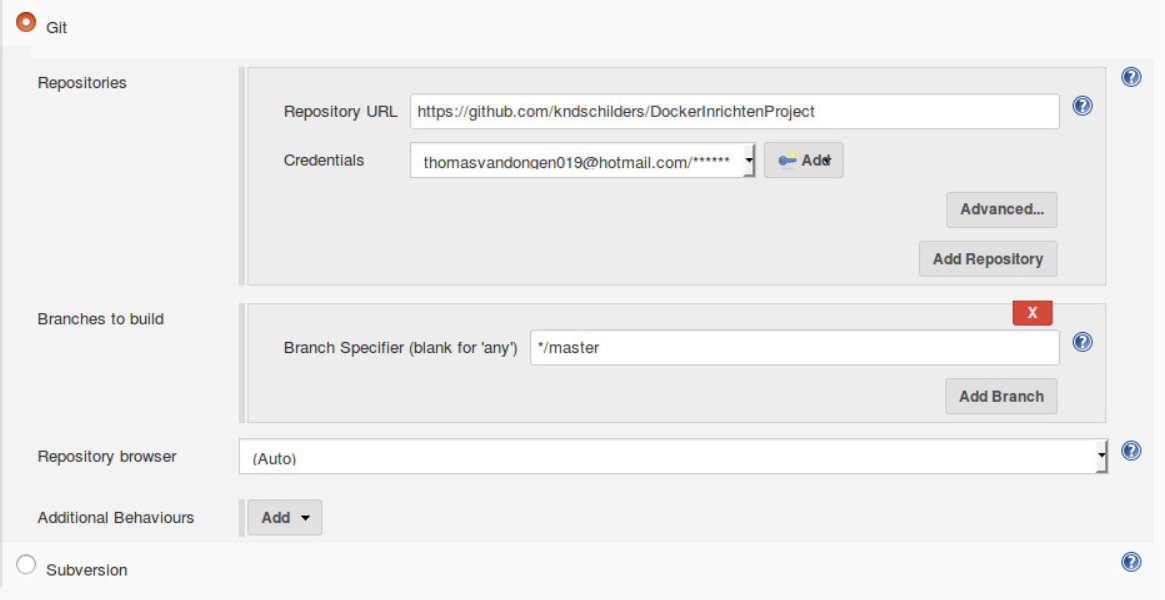
\includegraphics[width=1.0\textwidth]{images/Jenkins-Github-2.PNG}
		\caption{GitHub instellen\label{fig:jenkins_config_repo_2}}
	\end{center}
\end{figure}

\noindent Met Maven kan de applicatie gebuild worden. Dit wordt gedaan door de commando's 'clean', 'install' en 'test' uit te voeren.

\begin{figure}[H]
	\begin{center}
		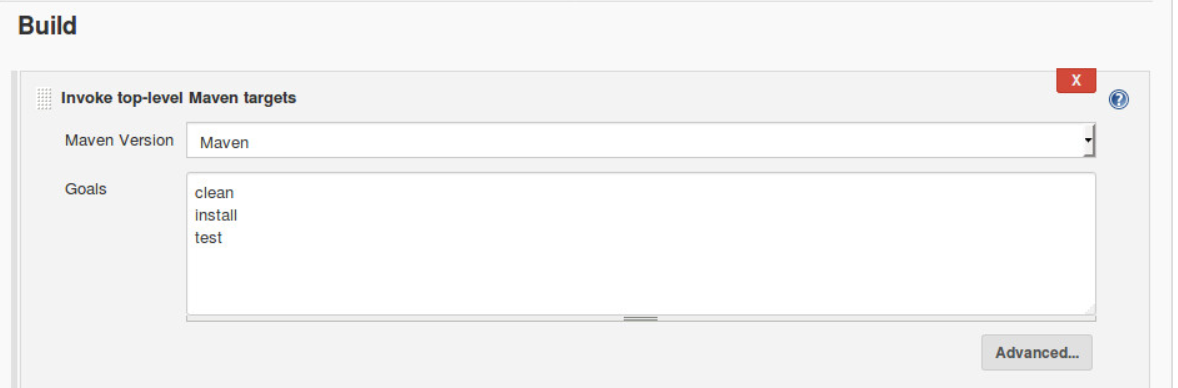
\includegraphics[width=1.0\textwidth]{images/Maven.PNG}
		\caption{Maven instellen\label{fig:jenkins_maven}}
	\end{center}
\end{figure}

\noindent Als laatste moeten er mail notifications ingesteld worden. Hier wordt simpelweg een email-adres ingevoerd. Als Jenkins iets te melden heeft wordt er naar dit email-adres een mailtje verstuurd.

\begin{figure}[H]
	\begin{center}
		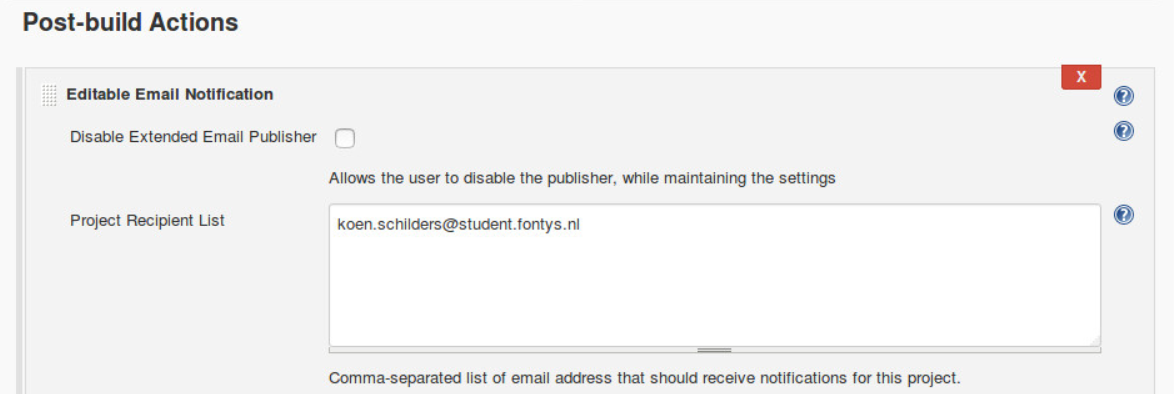
\includegraphics[width=1.0\textwidth]{images/Postbuildaction.PNG}
		\caption{Email notifications instellen\label{fig:jenkins_config_email_notifications}}
	\end{center}
\end{figure}

\noindent Na het opslaan van deze aanpassingen is Jenkins correct geconfigureerd.

\pagebreak
\subsection{Deployment container}
\noindent De Jenkins container is klaar, en de image (een war-file) wordt in de shared volume folder gezet. Nu moet de war-file draaien in een andere container.

We hebben gekozen om de war-file in een GlassFish-container te draaien. We pullen eerst een GlassFish-image:

\begin{lstlisting}[language=Bash]
docker oracle/glassfish:latest
\end{lstlisting}

\noindent Er moet een GlassFish-container gemaakt worden, welke gebaseert is op de GlassFish-image. Deze container moet toegang krijgen tot de war file gemaakt door de Jenkins container, omdat deze war gepubliseert gaat worden. Daarnaast moeten de IP's gemapped worden zodat we de gepubliseerde applicatie kunnen bereiken vanaf het host systeem. Dit kan allemaal in één run-commando:

\begin{lstlisting}[language=Bash]
docker run -i -t -p 4848:4848 -p 8181:8181 -v "/var/lib/docker/volumes/jenkins_home/_data/workspace/SOP6 Docker/target":/glassfish5/glassfish/domains/domain1/autodeploy oracle/glassfish:latest
\end{lstlisting}

\noindent Met dit commando wordt een nieuwe GlassFish-container aangemaakt. De IP's zijn gemapped, zodat we vanaf de host-VM de draaiende applicatie op GlassFish kunnen bereiken. Het volume waar de war-file staat is meegegeven, zodat de GlassFish-container de bestanden tot zijn beschikking heeft. Omdat de volume gemapped is naar de 'autodeploy' folder wordt de applicatie automatisch gedeployed. Het resultaat is te zien in Figure \ref{fig:glassfish_application}.

\begin{figure}[H]
	\begin{center}
		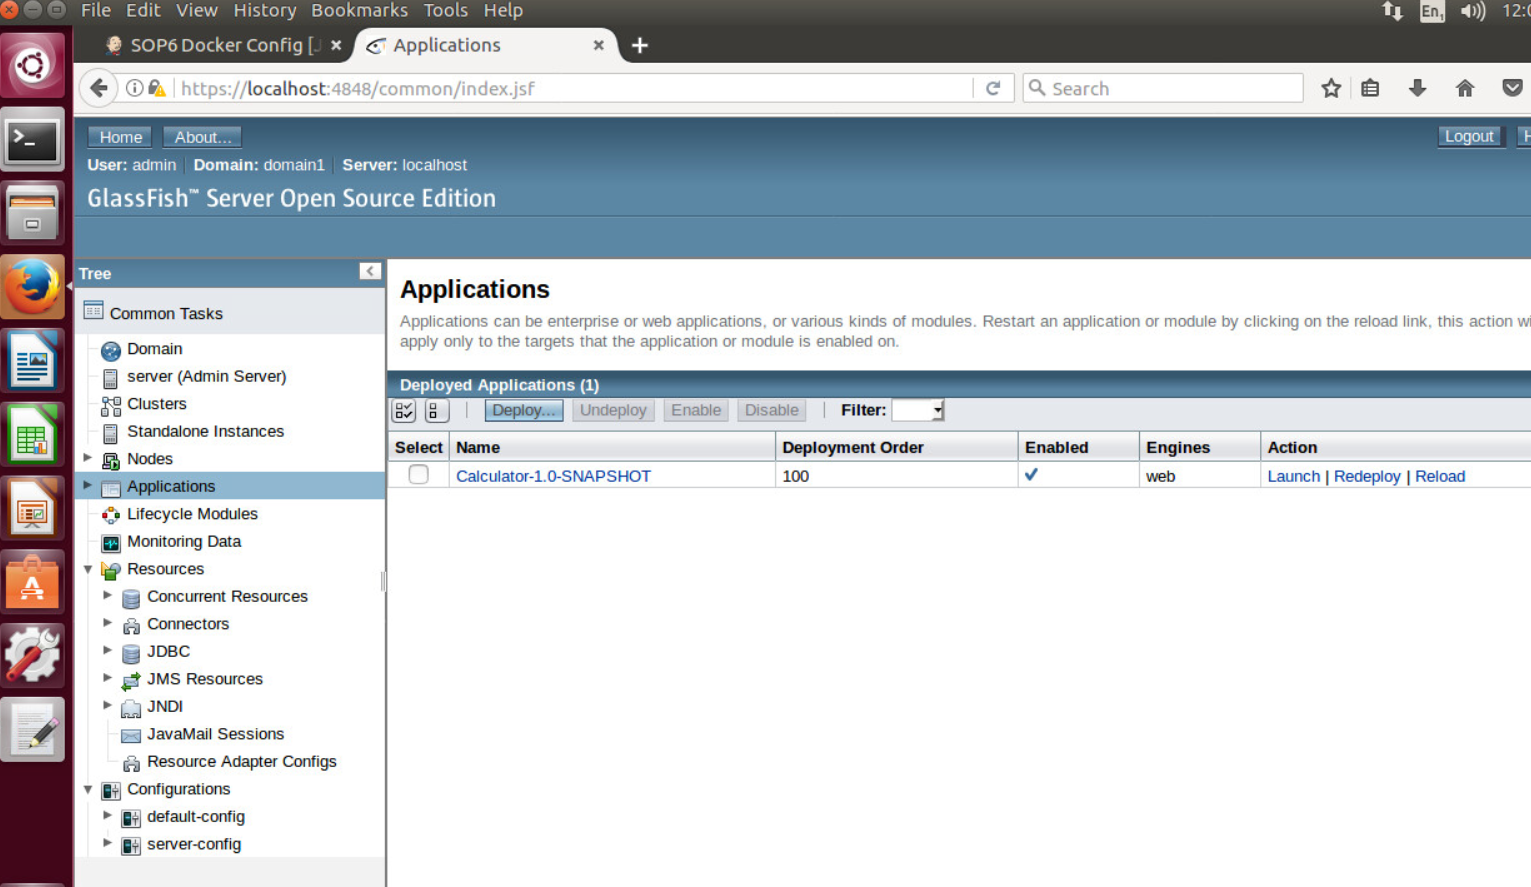
\includegraphics[width=1.0\textwidth]{images/applications_glassfish.png}
		\caption{GlassFish heeft de war gevonden\label{fig:glassfish_application}}
	\end{center}
\end{figure}

Nu hebben we een werkende CI/CD pipeline met gebruik van Docker containers. Er wordt automatisch een build getest en gemaakt als er wijzigingen op de master-branch van de repository worden gepushed. Vervolgens kan met het 'docker run' commando van hierboven de applicatie worden gehost in een container. Het is mogelijk om meerdere instanties van de GlassFish-container te runnen, waardoor het hosten van de applicatie schaalbaar is:

\begin{lstlisting}[language=Bash]
docker run -d -p 8181:8181 -v "/va.. oracle/glassfish:latest
docker run -d -p 8182:8181 -v "/va.. oracle/glassfish:latest
\end{lstlisting}

% Sources
\begin{thebibliography}{9}
	\bibitem{jenkins_documentation}
		Tom Hipkin,
		\textit{Official Jenkins Docker image},
		24 januari 2018,
		\url{https://github.com/jenkinsci/docker/blob/master/README.md}
\end{thebibliography}
\end{document}